
% !TeX program = xelatex
% !TEX root = main.tex
% !TeX encoding = UTF-8
\documentclass[10.5pt,compsoc]{CjC}
%\usepackage{CJKutf8}
%\usepackage{CJK}
\usepackage{graphicx}
\usepackage{footmisc}
\usepackage{subfigure}
\usepackage{url}
\usepackage{multirow}
\usepackage[noadjust]{cite}
\usepackage{amsmath,amsthm}
\usepackage{amssymb,amsfonts}
\usepackage{booktabs}
\usepackage{color}
\usepackage{ccaption}
\usepackage{booktabs}
\usepackage{float}
\usepackage{fancyhdr}
\usepackage{caption}
\usepackage{xcolor,stfloats}
\usepackage{comment}
\setcounter{page}{1}
\graphicspath{{figures/}}
\usepackage{cuted}%flushend,
\usepackage{captionhack}
\usepackage{epstopdf}


%===============================%

%\firstfootname{ \quad \quad }
\headevenname{\mbox{\quad} \hfill  \mbox{\zihao{-5}{\songti  计\quad \quad 算\quad \quad 机\quad \quad 学\quad \quad 报 } \hspace {50mm} \mbox{\songti 2024 年 }}}%
\headoddname{\songti
彭渤生, 邢骏洋,王~~京,肖家生:模糊测试技术中测试生成技术综述}%

%footnote use of *
\renewcommand{\thefootnote}{\fnsymbol{footnote}}
\setcounter{footnote}{0}
\renewcommand\footnotelayout{\zihao{5-}}

\newtheoremstyle{mystyle}{0pt}{0pt}{\normalfont}{1em}{\bf}{}{1em}{}
\theoremstyle{mystyle}
\renewcommand\figurename{figure~}
\renewcommand{\thesubfigure}{(\alph{subfigure})}
\newcommand{\upcite}[1]{\textsuperscript{\cite{#1}}}
\renewcommand{\labelenumi}{(\arabic{enumi})}
\newcommand{\tabincell}[2]{\begin{tabular}{@{}#1@{}}#2\end{tabular}}
\newcommand{\abc}{\color{white}\vrule width 2pt}
\makeatletter
\renewcommand{\@biblabel}[1]{[#1]\hfill}
\makeatother
\setlength\parindent{2em}
%\renewcommand{\hth}{\heiti }
%\renewcommand{\htss}{\begin{CJK*}{UTF8}{song}}


\begin{document}
\hyphenpenalty=50000
\makeatletter
\newcommand\mysmall{\@setfontsize\mysmall{7}{9.5}}
\newenvironment{tablehere}
  {\def\@captype{table}}

\let\temp\footnote
\renewcommand \footnote[1]{\temp{\zihao{-5}#1}}


\thispagestyle{plain}%
\thispagestyle{empty}%
\pagestyle{CjCheadings}

\begin{table*}[!t]
\vspace {-13mm}
\begin{tabular}{p{168mm}}
\zihao{5-}
\songti 
计\quad 算\quad 机\quad 学\quad 报\hfill CHINESE JOURNAL OF COMPUTERS\\
\hline\\[-4.5mm]
\hline\end{tabular}

\centering
\vspace{11mm}
\heiti  
{\zihao{2} 基于变异的测试用例生成技术综述 }

\vskip 5mm

{\zihao{3} \fangsong 
彭渤生$^{1)}$\quad  邢骏洋$^{1)}$ \quad 王~~京$^{1)}$ \quad 肖家生$^{1)}$
 }

\vspace{5mm}
\zihao{6}{\songti 
$^{1)}$(南京大学软件学院, 南京, 210093)}

\vskip 5mm
{\centering
\begin{tabular}{p{160mm}}
\zihao{5-}{
\setlength{\baselineskip}{16pt}\selectfont{
% TODO: 中文摘要内容
\noindent\heiti 摘\quad 要\quad   \songti  
*中文摘要内容置于此处(英文摘要中要有这些内容),字体为小5号宋体。摘要贡献部分,要有数据支持,不要出现``...大大提高''、``...显著改善''等描述,正确的描述是``比{\ldots}提高X{\%}''、
``在{\ldots}上改善X{\%}''。*摘要

 \par}}\\[2mm]

% TODO: 中文关键字
\zihao{5-}{\noindent
\heiti 关键词  \quad \songti  {*关键词(中文关键字与英文关键字对应且一致,应有5-7个关键词);关键词;关键词;关键词*  }
 
}\\[2mm]
\zihao{5-}{\heiti 中图法分类号 	\songti  
TP \rm{\quad \quad \quad     }
\heiti DOI号: \songti  
*投稿时不提供DOI号 }
\end{tabular}}

\vskip 7mm

\begin{center}
\zihao{3}{ {\heiti A Survey for Test Generation Techniques Based on Mutation Technology
}}\\
\vspace {5mm}
\zihao{5}{ {\heiti PENG Bo-Sheng$^{1)}$ XING Jun-Yang$^{1)}$ WANG Jing$^{1)}$ XIAO Jia-Sheng$^{1)}$
}}\\
\vspace {2mm}
\zihao{6}{\heiti {$^{1)}$(Software Institute, Nanjing University, Nanjing 210093, China)} }

\end{center}

\begin{tabular}{p{160mm}}
\zihao{5}{
\setlength{\baselineskip}{18pt}\selectfont{
{\bf Abstract}\quad \begin{heiti} (\textbf{500英文单词,内容包含中文摘要的内容}).
字体为Times new Roman,字号5号* Abstract \end{heiti}
\par}}\\

\setlength{\baselineskip}{18pt}\selectfont{
% TODO: 英文摘要内容
\zihao{5}{\noindent Do not modify the amount of space before and after the artworks. One- or two-column format artworks are preferred. and Tables, create a new break line and paste the resized artworks where desired. Do not modify the amount of space before and after the artworks. One- or two-column format artworks are preferred. All Schemes, Equations, Figures, and Tables should be mentioned in the text consecutively and numbered with Arabic numerals, and appear below where they are mentioned for the first time in the main text. To insert Schemes, Equations, Figures, and Tables, create a new break line and paste the resized artworks where desired. Do not modify the amount of space before and after the artworks. One- or two-column format artworks are preferred.Do not modify the amount of space before and after the artworks. One- or two-column format artworks are preferred. and Tables, create a new break line and paste the resized artworks where desired. Do not modify the amount of space before and after the artworks. One- or two-column format artworks are preferred. All Schemes, Equations, Figures, and Tables should be mentioned in the text consecutively and numbered with Arabic numerals, and appear below where they are mentioned for the first time in the main text.

\vspace {5mm}
% TODO: 英文关键字
{\bf Keywords}\quad \heiti 中文关键字与英文关键字对应且一致,\textbf{不要用英文缩写});
key word; key word; key word* *字体为5号Times new Roman * Key words }\par}
\end{tabular}

\setlength{\tabcolsep}{2pt}
\begin{tabular}{p{0.05cm}p{16.15cm}}
\multicolumn{2}{l}{\rule[4mm]{40mm}{0.1mm}}\\[-3mm]
&\begin{songti}
% TODO: 作者信息
彭渤生,性别男,xxxx年生,学位(或目前学历),职称,是/否计算机学会(CCF)会员(提供会员号),主要研究领域为*****、****.E-mail: **************.邢骏洋,性别男,2004年生,本科生,职称,主要研究领域为图形化界面软件测试.E-mail: xingjunyang@smail.nju.edu.cn. 王京(通信作者),性别男,xxxx年生,学位(或目前学历),职称,是/否计算机学会(CCF)会员(提供会员号),主要研究领域为*****、****.E-mail: **************.肖家生男,性别,xxxx年生,学位(或目前学历),职称,是/否计算机学会(CCF)会员(提供会员号),主要研究领域为*****、****.E-mail: **************.
第1作者手机号码(投稿时必须提供,以便紧急联系,发表时会删除): … …, E-mail: … …*此部分6号宋体*
\end{songti}
\end{tabular}\end{table*}
\clearpage\clearpage
\begin{strip}
\vspace {-13mm}
\end{strip}
    \linespread{1.15}
\heiti 
\zihao{5}
\vskip 1mm

% TODO: 正文内容
\section{引言}
\songti
随着信息化的发展,软件系统的数量、规模和复杂度不断增大。在软件系统的开发过程的,软件测试与漏洞发掘总是至关重要的。遗留的漏洞可能遭受黑客的利用,造成重大的经济损失和信息泄露。例如,2024年7月美国网络安全公司CrowdStrike发布异常更新,导致全球超过850万台Windows设备陷入“蓝屏死机”循环,甚至无法启动。此事件导致银行、航空、电信等多个关键行业的业务中断,重创了包括澳大利亚政府在内的多个组织的基础设施。尽管这一问题迅速被修复,但它揭示了软件更新测试不足和对关键依赖过于集中所带来的高风险\cite{Jones}。另一个例子是2017年的勒索软件WannaCry攻击,这次攻击影响了大约150个国家的约23万至30万台计算机,估计全球经济损失达40至80亿美元。 这次攻击发生的原因是用户没有使用 Microsoft Windows 发布的安全补丁更新他们的系统\cite{Maria}。

为了减少软件漏洞带来的损害,各类软件测试技术蓬勃发展,其中模糊测试已成为当前最流行的方法之一。模糊测试是一种通过随机或半随机的方式生成测试用例,将其输入到目标系统后监听异常结果来发现安全漏洞的安全检测技术。在模糊测试的流程中,输入生成的主要作用是通过不同策略生成能够引发程序异常行为、潜在漏洞或者新代码路径的输入数据。这类样例也被称为“有趣”的样例。确保样例的“有趣”才能保证在后续的测试运行时高效,覆盖率高。从而提高程序的安全性与鲁棒性。

模糊测试输入生成通常遵循以下流程:首先,选择模糊测试目标。可以是源代码、二进制代码,应用程序等。然后必须了解目标接受的输入格式和协议,确保输入数据服务目标预期。生成测试用例时,可以参考之前经过验证的有趣的用例集,或者直接生成新用例。用例的生成策略主要有随机生成和基于语法生成。当测试执行完成之后,对于触发异常的用例,可以保存以供重用或突变后产生新的测试样例。 

基于突变的随机生成测试用例\cite{LibFuzzer, Chenyang, Shuitao}是一种常见的技术,通过注入随机且不可预测的输入来检测应用程序中的漏洞和缺陷。这种方法有助于生成在代码演化或测试阶段尚未探索的新测试用例。然而,随机生成的局限性在于其变异能力的边界限制 - 它只能在现有种子语料库的范围内生成测试用例。如果种子语料库中不包含特定的输入模式或数据结构,就无法生成探索这些特定条件下应用程序行为的测试用例。然而,基于变异的技术可以在更高的抽象级别上操纵输入数据。它可以通过转换输入数据结构(添加/删除)而不是随机更改单个字节来生成新的测试用例。

一个扩展的想法是基于语法生成测试用例\cite{Cornelius, Martin}来为基于生成和变异的模糊测试其提供更好的能力。这种方法利用目标程序接受的输入的形式化语法规范来指导测试用例的生成。通过遵循预定义的语法规则,可以生成在语法上有效的输入,提高测试的效率。与随机生成相比,基于语法的方法能够更好地处理具有复杂输入格式的程序,如编译器、解释器等。此外,将代码片段内联到语法结构中有助于探索代码中的复杂路径,并通过做出使用上下文无关语法无法执行的精确决策来执行复杂操作。但是,它需要对输入语言语法有深入的了解,并且可能需要为复杂或专有的输入语言开发自定义语法。然而,生成的测试用例可能并不总是包含意外或恶意内容,需要进一步变异或生成以增加发现漏洞和错误的可能性。
\vspace {10mm}

\section{基础变异策略}

\subsection{AFL的经典变异策略及其变种}



\section{高级变异技术}

\subsection{基于程序分析的变异}
在模糊测试输入生成的评估中,如何提高路径尤其是复杂深层次的路径以及提高测试用例的生成效率是非常重要的参考指标。AFL作为里程碑式的工具通过反馈机制实现了简单易用以及相对高效的随机生成机制。但是AFL仍然存在着复杂和深层次路径难以探索、针对复杂输入格式时难以生成符合规范的输入和路径探索相对随机等问题。在后期发展的各种框架工具中,基于程序分析的符号执行和污点跟踪技术很好的解决了上述问题。

魔法数字和嵌套校验和也是模糊测试中常见的两大难题。魔法数字通常指的是程序中用于验证输入完整性的特定值,而嵌套校验和则涉及到更复杂的数据完整性验证,如在多层数据结构中计算和比较校验和。这些校验机制的存在显著增加了模糊测试的难度,因为随机生成的输入很难通过这些校验,从而导致测试覆盖率降低。为了克服这些难题,研究人员开发了多种技术,包括基于污点分析的方法和基于符号执行的方法,以提高模糊测试的效率和效果。这些技术通过分析程序的行为和输入数据的流向,自动生成能够通过校验的测试用例,从而深入探索程序的状态空间,发现潜在的安全漏洞。

TaintScope\cite{TaintScope}是一个经典的基于动态污点分析和符号执行技术的模糊测试工具,它在无需访问源代码或精确了解平台指令集的情况下,自动检测输入中的校验字段并精确定位程序中的校验基于完整性检查。该工具的主要贡献在于其能够通过控制流修改来绕过这些校验,从而显著提高模糊测试的覆盖率和效率。TaintScope不仅能够识别和绕过校验检查,还能自动修复生成输入中的校验值,使其能够触发潜在的漏洞。这一方法有效地结合了污点跟踪和符号执行的优点。

GreyOne\cite{GREYONE}是一种先进的数据流敏感模糊测试技术,其关键技术包括轻量级且准确的污点推断FTI、基于污点的输入优先级模型以及约束一致性引导的进化策略。FTI通过监控输入变异时变量值的变化来推断变量的污点状态,这种方法不仅避免了传统污点分析中的劳动密集型工作,而且提高了污点分析的准确性和运行时效率。GreyOne利用FTI提供的污点信息来确定哪些输入字节应该优先变异以及如何变异,以探索更多未触及的代码路径。此外,通过考虑污点变量与未触及分支中预期值的距离(即约束一致性),GreyOne能够调整其进化方向,更有效地探索难以到达的分支。这些技术的结合使得GreyOne在代码覆盖率和漏洞发现方面超越了多种现有的模糊测试工具,展现出其在模糊测试领域的显著优势。

T-Fuzz\cite{T-Fuzz}是一种基于程序变换的模糊测试方法,它通过移除目标程序中的输入检查来提高代码覆盖率。T-Fuzz利用覆盖引导的模糊测试生成输入,并在模糊测试无法触发新代码路径时,使用轻量级的动态追踪技术检测输入检查,然后将这些检查从目标程序中移除。这种方法允许之前被检查保护的代码被触发,从而有可能发现潜在的错误。T-Fuzz面临的挑战包括移除检查可能导致过度近似和误报,以及在变换程序中触发的崩溃输入可能不会在原始程序中触发错误。为了解决这些问题,T-Fuzz采用了基于符号执行的方法作为辅助的后处理步骤,以过滤掉误报并在原始程序中复现真正的错误。通过变换程序和输入变异,T-Fuzz能够覆盖更多的代码,并发现比现有技术更多的真实错误。

Angora是一种基于变异的模糊测试工具,它通过引入一系列关键技术来提高路径覆盖率,有效解决了路径约束问题。Angora的主要目标是在不使用符号执行的情况下,通过解决路径约束来增加分支覆盖。它采用了可扩展的字节级污点跟踪技术,这种技术通过跟踪输入字节如何流入程序中的每个路径约束,使得Angora能够只突变那些影响路径约束的字节,而不是整个输入,从而大幅减少了探索空间。此外,Angora还采用了基于梯度下降的搜索算法,这种算法在机器学习中非常流行,它避免了昂贵的符号执行,并且能够高效地解决路径约束。Angora还进行了类型和形状推断,这使得梯度下降算法能够更有效地搜索,因为它能够识别输入中哪些字节被集体用作单个值,并推断出这些值的类型。最后,Angora还探索了输入长度,因为某些程序状态只有在输入长度超过某个阈值时才会被探索,而Angora能够检测到这一点并适当增加输入长度。
\vspace {10mm}

\subsection{基于输入与程序状态对应关系的变异}
REDQUEEN\cite{redqueen}是一种新颖的模糊测试方法,它基于输入到状态的对应关系,以提高反馈驱动模糊测试的效率和效果。这种方法特别针对两个常见的模糊测试难题:魔术数字和(嵌套)校验和,这些问题通常需要复杂的程序分析技术,如污点跟踪和符号执行来解决。REDQUEEN通过在程序执行过程中观察输入与程序状态之间的直接对应关系,实现了一种轻量级且高效的解决方案,无需访问源代码或对平台指令集的精确语义。
	与前述两篇论文中提到的Angora和T-Fuzz相比,REDQUEEN在几个关键方面进行了改进和优化。首先,REDQUEEN不依赖于符号执行或污点跟踪,这使得它在大型二进制应用程序和未知环境中更容易扩展且高效。其次,REDQUEEN通过“着色”输入和程序追踪,创建了一种轻量级的污点跟踪近似方法,从而有效地识别和解决魔术数字和校验和问题。此外,REDQUEEN还能够自动修复通过校验和的输入,而无需人工干预或复杂的符号执行方法,这在Angora和T-Fuzz中是不具备的。
  \vspace {10mm}
  
\subsection{基于路径感知的变异}
PATA\cite{PATA}的主要贡献在于其创新性地将路径感知的污点分析技术融入到模糊测试中,显著提升了对复杂软件漏洞的发现能力。传统的模糊测试技术依赖于随机或基于覆盖率的输入变异,而PATA通过精确识别输入数据与程序执行路径中特定变量的依赖关系,实现了对输入数据的智能变异。这种路径感知的污点分析能够区分同一变量在不同执行路径上的多次出现,解决了传统技术在面对循环和多次函数调用时的局限性,从而避免了过污点和欠污点的问题。PATA首先通过构建代表性变量序列(RVS),记录变量在执行路径上的所有出现及其值,然后通过输入微调并匹配RVS来识别影响这些变量值的关键输入字节。这种方法不仅提高了变异的针对性,还增强了模糊测试在探索程序逻辑和发现新漏洞方面的效率。
此外,PATA的先进性还体现在其路径导向的变异策略上。利用路径感知污点分析的结果,PATA能够精确地识别出对于每个变量出现至关重要的输入字节,并结合变量的特征和值,选择最合适的变异方法来绕过约束,探索程序状态空间中未被覆盖的分支。这种策略使得PATA在面对复杂的程序逻辑和深层次的漏洞时,能够更加高效地触发新的执行路径和基本块,从而发现更多的独特路径和基本块覆盖。在多个基准测试和真实世界的项目中,PATA相较于现有的先进模糊测试工具,展现出了显著的性能提升,不仅在路径和基本块覆盖上超越了其他工具,而且在漏洞发现方面也表现出色,这进一步证明了PATA在模糊测试领域的创新性和先进性。
\vspace {10mm}

\section{定向与智能变异}

\subsection{定向模糊测试}

定向模糊测试(Directed Fuzzing)是一种有目标性的模糊测试方法,其核心思想是针对程序中特定的代码位置或功能进行测试,通过各种策略引导测试过程到达目标位置,集中资源测试可能存在风险的区域。定向模糊测试的主要技术手段主要包含静态分析确定目标位置,符号执行计算路径约束,动态污点分析跟踪数据流以及启发式算法指导种子选择和变异。DGF是以启发式算法指导种子选择和变异的一个例子,它通过使用模拟退火算法为基础的功率调度,逐渐为接近目标位置的种子分配更多能量,同时减少远离目标的种子的能量,以此实现带有目标性的模糊测试。其主要的变异策略可以概括如下:
\begin{itemize}
\item 基于模拟退火的功率调度:AFLGo使用模拟退火算法动态调整每个种子的能量,优先考虑那些更接近目标位置的种子
\item 全局搜索:AFLGo实现了全局搜索,与AFL的局部搜索相比,能够更有效地接近全局最优解,即覆盖最多的目标位置
\item 并行搜索:AFLGo同时搜索所有目标,提高了搜索效率,并允许同时对多个目标进行模糊测试
\item 种子距离计算:AFLGo计算每个种子到目标位置的距离,并根据这个距离来调整种子的能量,使得更接近目标的种子获得更多的测试机会
\item 能量分配:AFLGo根据种子与目标位置的距离和当前时间来分配能量,确保在测试过程中,能量分配能够逐渐向目标位置倾斜
\end{itemize}

DGF同时还可以集成现有灰盒模糊测试,与现有的灰盒模糊测试工具(如AFL)集成,利用其轻量级的程序分析和覆盖信息来指导变异过程\cite{Böhme}。

\vspace {10mm}

\subsection{机器学习辅助}

机器学习技术在模糊测试领域的应用正在带来革新性的影响。通过对大量测试数据的学习和分析,ML可以帮助优化测试过程中的多个关键环节。在种子生成和选择方面,机器学习模型能够预测种子的质量和潜在价值,从而更智能地分配测试资源。在变异策略上,ML可以通过学习历史数据来识别最有效的变异模式,提高发现新执行路径的效率。在路径探索方面,机器学习算法能够分析程序结构特征,预测更可能存在漏洞的代码区域,从而指导测试过程更有针对性地进行探索。深度学习模型可以用于预测程序崩溃的概率,强化学习则可以持续优化测试策略。这些技术的应用大大提升了模糊测试的效率和效果。 Learn\&Fuzz的工作展示了机器学习在测试用例生成中的潜力。具体而言,Learn\&Fuzz采用了以下四种变异生成测试的方式\cite{Godefroid}:

\begin{itemize}
  
  \item NoSample(无采样: 使用学习到的分布来贪婪地预测给定前缀下的最佳字符。这会导致生成的PDF对象最有可能是格式良好且一致的。
  \item Sample(采样): 使用学习到的分布来采样序列中的下一个字符,而不是选择预测最高的字符。这种采样策略能够通过结合模型从训练语料中学习到的各种模式,生成多样化的新PDF对象。
  \item SampleSpace(样本空间):这种采样策略结合了Sample和NoSample策略。它只在当前缀序列以空白字符结束时才采样分布来生成下一个字符,而在标记内部(即前缀以非空白字符结束时)使用分布中最佳预测的字符,类似于NoSample策略。这种策略预期会生成比Sample策略更多格式良好的PDF对象,因为采样被限制在仅在空白字符后进行。
  \item SampleFuzz(采样模糊): 新的算法,用于在采样新对象的同时进行模糊测试。使用学习到的模型生成新的PDF对象实例,同时引入异常以测试错误处理代码。SampleFuzz算法根据学习到的分布决定在何处模糊值。如果在特定时间戳t,模型对于某个字符c的预测概率p(c)高于用户提供的阈值pt,算法将选择一个概率最低的字符c'来替换c。这种修改(模糊)仅在随机硬币投掷的结果pfuzz高于输入参数tfuzz时发生,允许用户进一步控制模糊字符的概率。通过学习已有样本的特征

\end{itemize}

不过,机器学习辅助的模糊测试也面临一些挑战。首先是获取足够的高质量训练数据比较困难,其次是需要在实时性要求和推理开销之间找到平衡。此外,如何提升模型的泛化能力,以及如何更好地将ML技术与传统模糊测试方法融合,都是需要进一步研究的问题。尽管如此,机器学习在模糊测试中的应用前景仍然十分广阔。随着算法和硬件的不断进步,相信这种结合将会产生更多创新性的成果。

\clearpage\clearpage
% TODO: 正文内容结束
% 以下是可参考的用法
% \section{一级标题*字体为4号黑体*标题1}
% \textbf{对投稿的基本要求}:
 
% \songti  
% (1) 研究性论文主体应包括引言(重点论述研究的科学问题、意义、解决思路、价值、贡献等)、相关工作(为与引言部分独立的一个章节)、主要成果论述、关键实现技术、验证(对比实验或理论证明)、结论(结束语)等内容;系统实现或实验应有关键点的详细论述,以便读者能够重复实现论文所述成果。实验应有具体的实验环境设置、全面细致的数据对比分析。

% (2) 综述应包括引言、问题与挑战、研究现状分析、未来研究方向、结论等内容。以分析、对比为主,避免堆砌文献或一般性介绍、叙述。

% (3) 定理证明、公式推导、大篇幅的数学论述、原始数据,放到论文最后的附录中。

% {\bf 稿件提交时的基本要求:}

% (1) 本模板中要求的各项内容正确齐全,无遗漏;

% (2) 语句通顺,无中文、英文语法错误,易于阅读理解,符号使用正确,图、表清晰无误;

% (3) 在学术、技术上,论文内容正确无误,各项内容确定。

% \vspace {10mm}

% {\heiti \subsection{二级标题 *字体为5号黑体*标题2} }
% \subsubsection{三级标题 *字体为5号宋体*标题3}
% *正文部分, 字体为5号宋体* 正文文字

% \textbf{正文文字要求语句通顺,无语法错误,结构合理,条理清楚,不影响审稿人、读者阅读理解全文内容。以下几类问题请作者们特别注意}:

% 1) 文章题目应明确反映文章的思想和方法;文字流畅,表述清楚;

% 2) 中文文字、英文表达无语法错误;

% 3) 公式中无符号、表达式的疏漏,没有同一个符号表示两种意思的情况;

% 4) 数学中使用的符号、函数名用斜体;

% 5) 使用的量符合法定计量单位标准;

% 6) 矢量为黑体,标量为白体;

% 7) 变量或表示变化的量用斜体;

% 8) 图表规范,量、线、序无误,位置正确(图表必须在正文中有所表述后出现,即{\ldots}如图1所示)(注意纵、横坐标应有坐标名称和刻度值)。

% 9) 列出的参考文献必须在文中按顺序引用,即参考文献顺序与引用顺序一致,各项信息齐全(格式见参考文献部分);

% 10) 首次出现的缩写需写明全称,首次出现的符号需作出解释。

% 11) 图的图例说明、坐标说明全部用中文或量符号。

% \textbf{12) 图应为矢量图。}

% 13) 表中表头文字采用中文。

% 14) 公式尺寸:

% 标准:10.5磅

% 下标/上标:5.8磅

% 次下标/上标:4.5磅

% 符号:16磅

% 次符号:10.5磅

% 15) 组合单位采用标准格式,如:``pJ/bit/m$^{4}$''应为 ``pJ/(bit$\cdot
% $m$^{4})$''

% {\heiti\textbf{定理1}. }\quad ******. *定理内容.*

% [``定义''、``假设''、``公理''、``引理''等的排版格式与此相同,详细定理证明、公式可放在附录中]

% { \fangsong 证明 }.\quad  *证明过程.* [``例 x''等的排版格式相同]

% \rightline {证毕.}

% \begin{figure}[htbp]
% \centerline{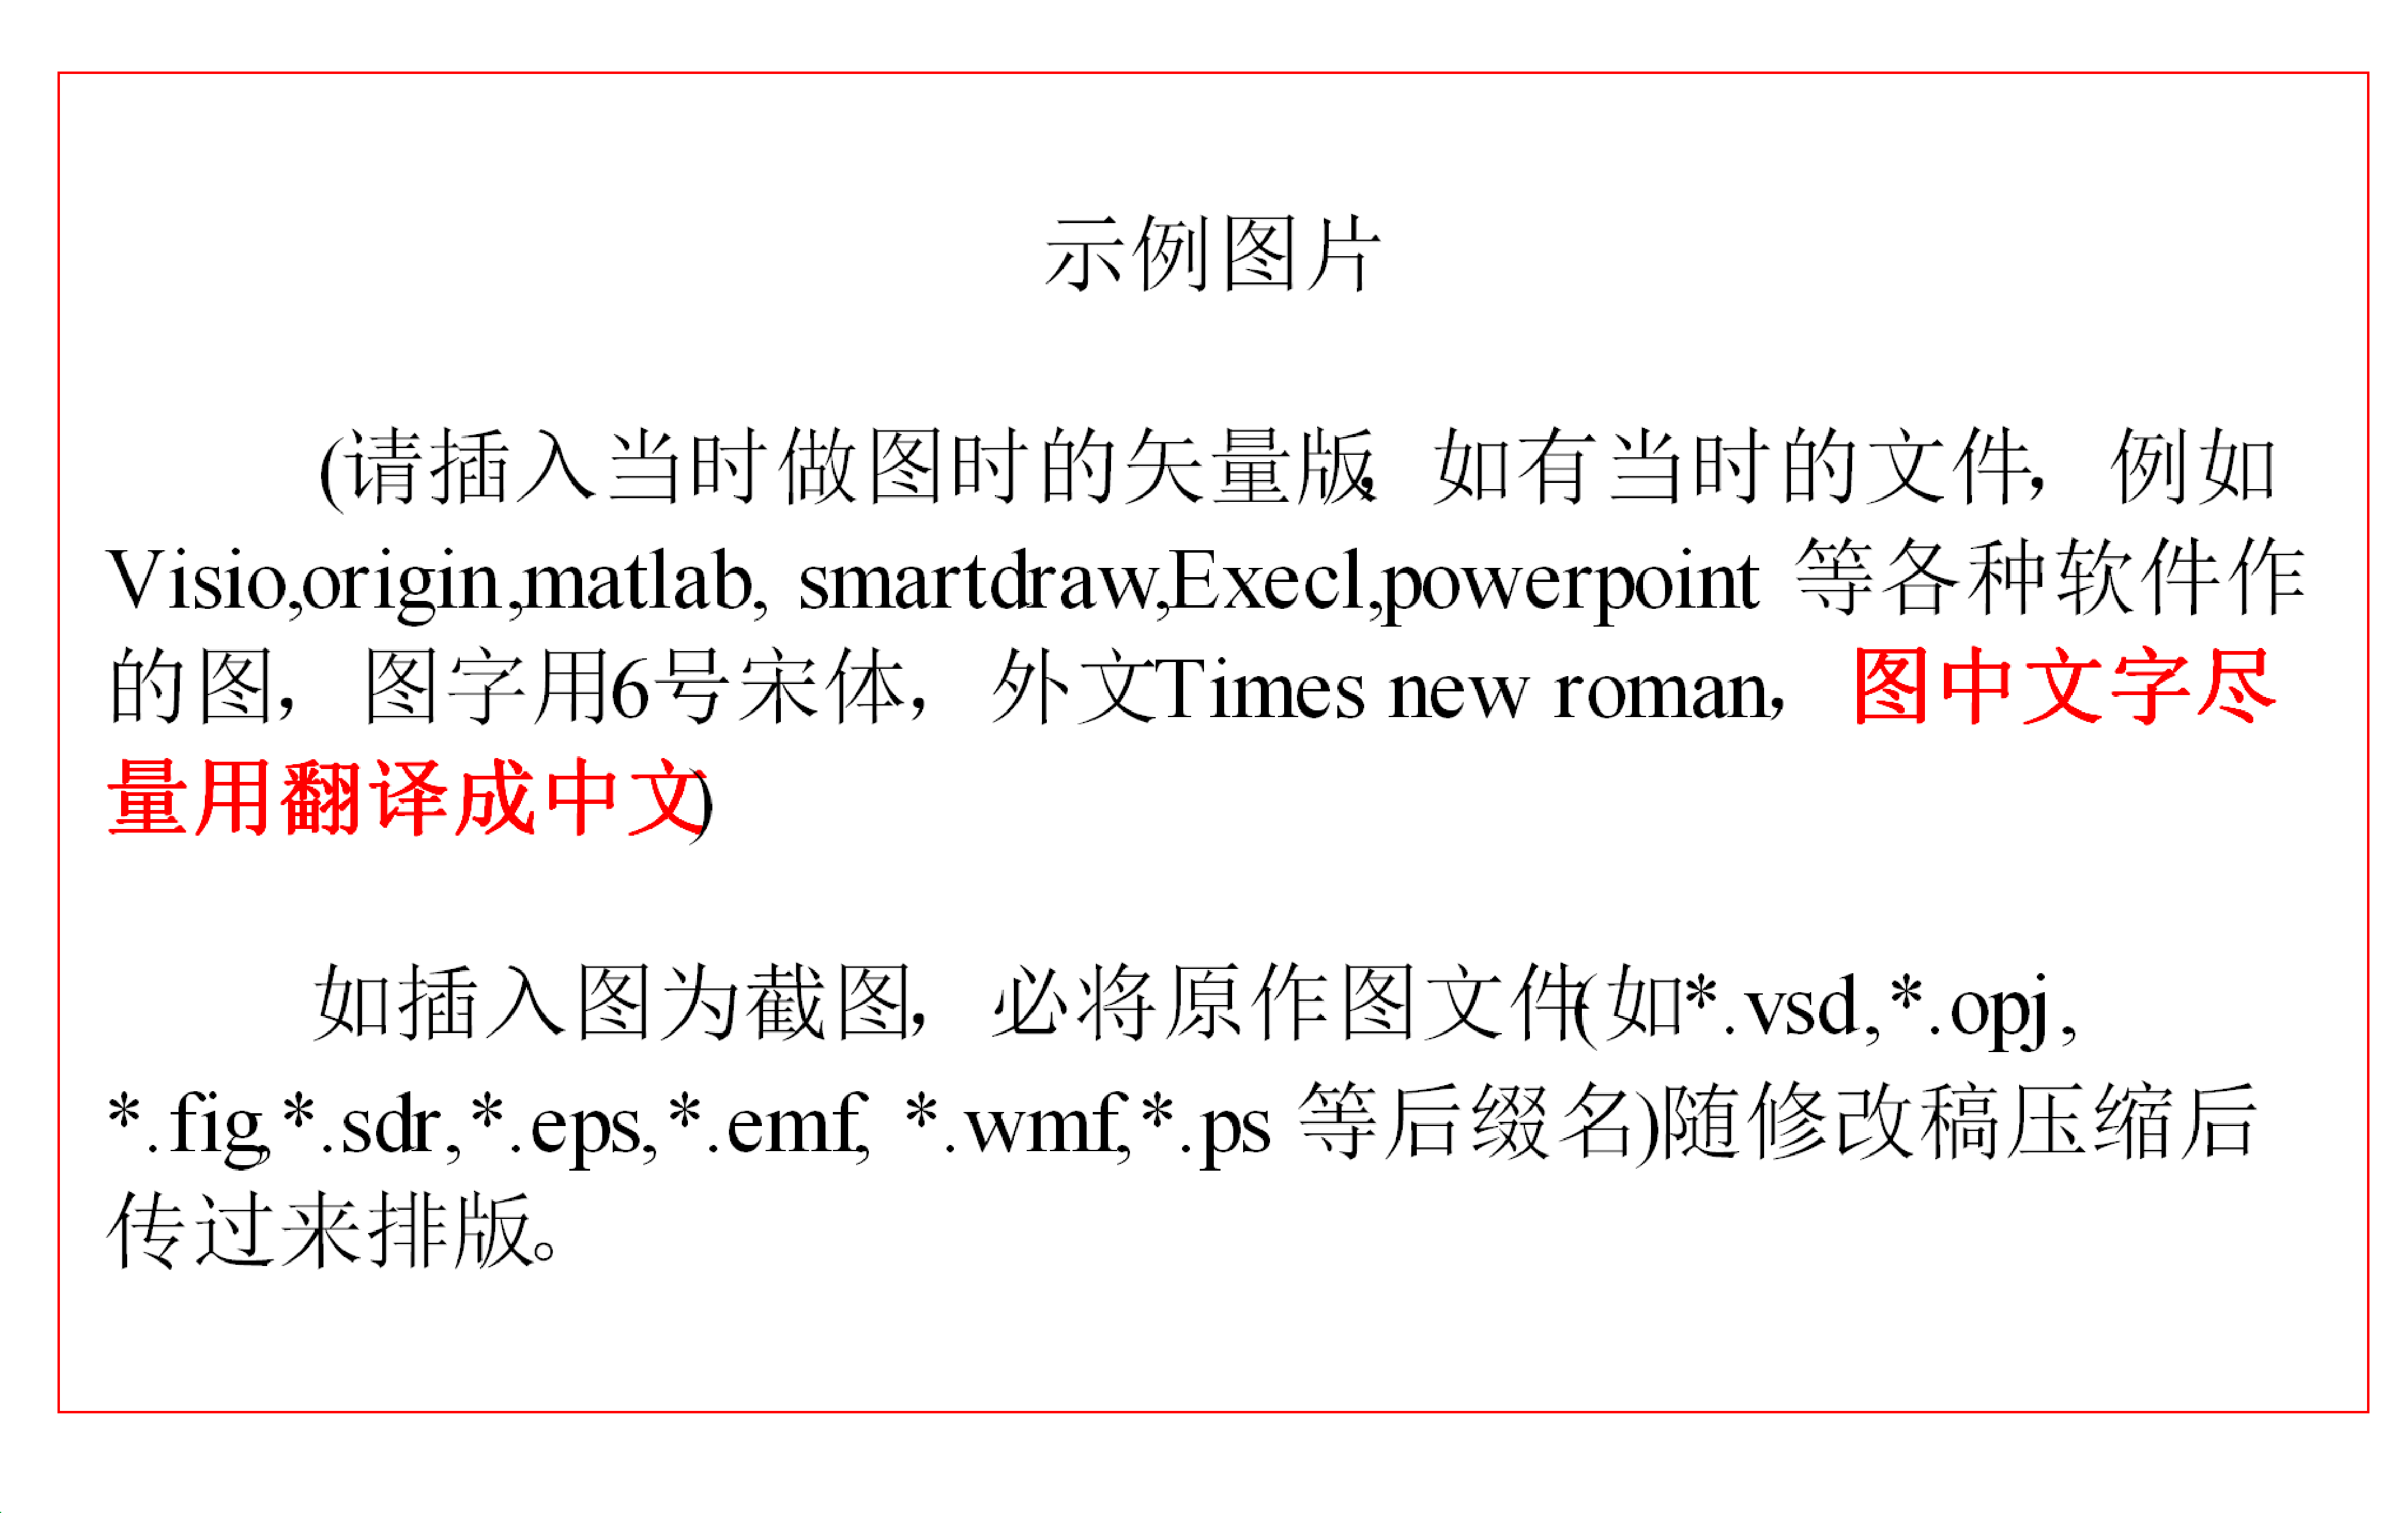
\includegraphics[width=3.15in,height=1.98in]{CJC1.pdf}}
% 图X\quad  图片说明 *字体为小5号,图片应为黑白图,图中的子图要有子图说明*
% \label{fig1}
% \end{figure}

% \begin{table}[htbp]
% \centering {\heiti 表X\quad 表说明 *表说明采用黑体* }
% \vspace {-2.5mm}
% \begin{center}
% \begin{tabular}{ll}
% \toprule
% *示例表格*&*第1行为表头,表头要有内容* \\
% \hline
% &
%  \\
% &
%  \\
% &
%  \\
% &
%  \\
% \bottomrule
% \end{tabular}
% \label{tab1}
% \end{center}
% \end{table}

% \heiti 过程X. \quad 过程名称

% {\zihao{5-}*《计算机学报》的方法过程描述字体为小5号宋体,IF、THEN等伪代码关键词全部用大写字母,变量和函数名称用斜体*}


% \heiti 算法\textbf{Y} .\quad 算法名称.
% \zihao{5-}{

% \noindent 输入:{\ldots} {\ldots}

% \noindent 输出:{\ldots} {\ldots}

% *《计算机学报》的算法描述字体为小5号宋体, IF、THEN等伪代码关键词全部用大写字母,变量和函数名称用斜体*}

\clearpage\clearpage


% TODO: 参考文献、致谢、附录、作者简介
\vspace {3mm}
\zihao{5}{
\noindent \heiti 致\quad 谢 \quad  \kaishu   *致谢内容.* 致谢 }

\vspace {5mm}
\centerline
{\zihao{5}
\heiti 参~考~文~献 }

\begin{thebibliography}{99}
\zihao{5-}
\vspace{3mm}
	\bibitem{Jones}
  Jones, J. (2024, July 19). A 'blue screen of death loop': How a Crowdstrike update crashed Microsoft systems around the world. City AM. Retrieved from https://www.cityam.com
	\bibitem{Maria}
	 Maria F. Prevezianou. 2021. WannaCry as a Creeping Crisis. Springer International Publishing.
  \bibitem{LibFuzzer}
  LibFuzzer 2017. libFuzzer—A Library for Coverage-guided Fuzz Testing. Retrieved from https://llvm.org/docs/LibFuzzer.html
  \bibitem{Chenyang}
  Chenyang Lyu, Shouling Ji, Chao Zhang, Yuwei Li, Wei-Han Lee, Yu Song, and Raheem Beyah. 2019. MOPT: Optimized mutation scheduling for fuzzers. In Proceedings of the 28th USENIX Security Symposium, 1949–1966.
  \bibitem{Shuitao}
  Shuitao Gan, Chao Zhang, Peng Chen, Bodong Zhao, Xiaojun Qin, Dong Wu, and Zuoning Chen. 2020. GREYONE:
Data flow sensitive fuzzing. In Proceedings of the 29th USENIX Security Symposium, 2577–2594.
  \bibitem{Cornelius}
  Cornelius Aschermann, Tommaso Frassetto, Thorsten Holz, Patrick Jauernig, A.-R. Sadeghi, and Daniel Teuchert. 2019. NAUTILUS: Fishing for deep bugs with grammars. In Proceedings of the Network and Distributed System Security
Symposium (NDSS’19). 1–15.
  \bibitem{Martin}
  Martin Eberlein, Yannic Noller, Thomas Vogel, and Lars Grunske. 2020. Evolutionary grammar-based fuzzing. In Proceedings of the 12th International Symposium of Search-Based Software Engineering (SSBSE’20). Springer-Verlag, 105–120.
  \bibitem{Böhme}
  Böhme, M., Pham, V.-T., Nguyen, M.-D., and Roychoudhury, A. (2017). Directed Greybox Fuzzing. In Proceedings of the 2017 ACM SIGSAC Conference on Computer and Communications Security (CCS ’17). Dallas, TX, USA: Association for Computing Machinery. https://doi.org/10.1145/3133956.3134020
  \bibitem{Godefroid}
  Godefroid, P., Peleg, H., and Singh, R. (2017). Learn$\&$Fuzz: Machine Learning for Input Fuzzing. In Proceedings of the 32nd IEEE/ACM International Conference on Automated Software Engineering (ASE 2017). Urbana-Champaign, IL, USA: IEEE. 978-1-5386-2684-9/17
  \bibitem{redqueen}
  Aschermann, C., Schumilo, S., Blazytko, T., Gawlik, R., and Holz, T. (2019). REDQUEEN: Fuzzing with Input-to-State Correspondence. In Network and Distributed System Security (NDSS) Symposium (24-27 February 2019). San Diego, CA, USA. https://dx.doi.org/10.14722/ndss.2019.23371
  \bibitem{TaintScope}
  Wang, T., Wei, T., Gu, G., and Zou, W. (2010). TaintScope: A Checksum-Aware Directed Fuzzing Tool for Automatic Software Vulnerability Detection. In Proceedings of the 2010 IEEE Symposium on Security and Privacy (SP'10). https://doi.org/10.1109/SP.2010.37
  \bibitem{T-Fuzz}
  Peng, H., Shoshitaishvili, Y., and Payer, M. (2018). T-Fuzz: Fuzzing by Program Transformation. In 2018 IEEE Symposium on Security and Privacy (SP'18). https://doi.org/10.1109/SP.2018.00056
  \bibitem{GREYONE}
  Gan, S., Zhang, C., Qin, X., Wu, D., Zhao, B., Qin, X., and Chen, Z. (2020). GREYONE: Data Flow Sensitive Fuzzing. In Proceedings of the 29th USENIX Security Symposium (12-14 August 2020). USENIX Association. 
  \url{https://www.usenix.org/conference/usenixsecurity20/presentation/gan}
  \bibitem{PATA}
  Liang, J., Wang, M., Zhou, C., Wu, Z., Jiang, Y., Liu, J., Liu, Z., and Sun, J. (2022). PATA: Fuzzing with Path-Aware Taint Analysis. In 2022 IEEE Symposium on Security and Privacy (SP)
\end{thebibliography}

\begin{biography}[pbs.jpg]
\noindent
\textbf{PENG Bo-Sheng}\ \ Undergraduate Student. His research interests include \textbf{machine learning, fuzzing, and software security}.
\end{biography}

\vspace{10mm}
\begin{biography}[yourphotofilename.jpg]
\noindent
\textbf{XING Jun-Yang} Undergraduate Student. His research interests include \textbf{machine learning, fuzzing, and software security}.
\end{biography}
\vspace{10mm}

\begin{biography}[yourphotofilename.jpg]
  \noindent
  \textbf{WANG Jing} Undergraduate Student. His research interests include \textbf{machine learning, fuzzing, and software security}.
\end{biography}

\vspace{10mm}
\begin{biography}[yourphotofilename.jpg]
\noindent
\textbf{XIAO Jia-Sheng} Undergraduate Student. His research interests include \textbf{machine learning, fuzzing, and software security}.
\end{biography}

\vspace{10mm}

\begin{strip}
\end{strip}

\zihao{5}
\noindent \textbf{Background}

\zihao{5-}{
\setlength\parindent{2em}
*论文背景介绍为\textbf{英文},字体为小5号Times New Roman体*

论文后面为400单词左右的英文背景介绍。介绍的内容包括:

本文研究的问题属于哪一个领域的什么问题。该类问题目前国际上解决到什么程度。

本文将问题解决到什么程度。

课题所属的项目。

项目的意义。

本研究群体以往在这个方向上的研究成果。

本文的成果是解决大课题中的哪一部分,如果涉及863$\backslash $973以及其项目、基金、研究计划,注意这些项目的英文名称应书写正确。}
 
\end{document}


